\documentclass[main.tex]{subfiles}

\begin{document}

\section{9-point Laplacian}
This section will extend the implementation of the 5-point Laplacian to a 9-point stencil and discuss how to form the right hand side of the Poisson equation using the correction 3.19 from LeVeque to achieve $\mathcal{O}(h^4)$ convergence in terms of global error (methods to find it can be found in the appendix of LeVeque).

The spacial domain will be unit square defined as $[0,1] \times [0,1]$ and discretized to a regular grid with $m \times m$ interior points ($(m+2) \times (m+2)$ with boundaries). Dirichlet BC are prescribed everywhere on the boundary, but the method \texttt{form\_rhs(m,f,u)} will use the ``exact'' $u$ to calculate them for the sake of simplicity.

% The stencil
\subsection{9-point stencil}
Visualization of the stencil is shown in figure 3.1b of LeVeque and is achieved in a similar manner as the 5-point stencil, that is by replacing the derivatives with centered finite differences to get the discretization. Since the grid is uniform this leads to equation 3.10 (LV) for the 5-point stencil:
\begin{equation}
    \frac{1}{h^2}(u_{i-1,j} + u_{i+1,j} + u_{i,j-1} + u_{i,j+1} - 4u_{i,j}) = f_{i,j} = \nabla_5^2 u_{i,j}
\end{equation}
It can be seen that a ``cross'' like shape is used with the coefficients adding up to 0. As mentioned in the book, this stencil has some drawbacks so let's look at the 9-point one.

The approximation is given by
\begin{equation}
\begin{split}
    \nabla_9^2 u_{i,j} = \frac{1}{6h^2}(&4u_{i-1,j} + 4u_{i+1,j} + 4u_{i,j-1} + 4u_{i,j+1} \\
        &+ u_{i-1,j-1} + u_{i-1,j+1} + u_{i+1,j-1} + u_{i+1,j+1}\\
        &- 20u_{i,j}
    )
\end{split}
\end{equation}
in order to achieve the fourth-order accuracy a clever expansion is presented in LeVeque: the approximation is applied to the true solution and expanded into a Taylor series, with the dominant error term rewritten as $u_{xxxx} + 2u_{xxyy} + u_{yyyy} = \nabla^2 (\nabla^2 u) \equiv \nabla^4 u$. For Poisson equation $\nabla^2 u = f$, it is possible to further rewrite $u_{xxxx} + 2u_{xxyy} + u_{yyyy}$ as $\nabla^2 f$. Given these results, the dominant error term can be computed with just the knowledge of the function $f$. More so, if $f$ is \textit{zero} or a \textit{harmonic} function, then the aforemention term in the local truncation error disappears and the 9-point Laplacian yields a fourth order accurate discretization.

This approach can be extended for arbitary smooth functions $f$ by defining
\begin{equation}
    \nabla_9^2 u_{ij} = f(x_i, y_j) + \frac{h^2}{12} \nabla^2 f(x_i, y_j)
\end{equation}
to cancel out the $\mathcal{O}(h^2)$ terms and end up with $\mathcal{O}(h^4)$ as the local truncation error of this method. 

Particularly useful trick for numerical methods when the values of $f$ are only known at the grid points is by using the 5-point Laplacian as follows:
\begin{equation}
    \nabla_9^2 u_{ij} = f(x_i, y_j) + \frac{h^2}{12} \nabla_5^2 f(x_i, y_j).
\end{equation}
Having $\mathcal{O}(h^4)$ out of the way, it is possible to implement the \texttt{form\_rhs} method by using \texttt{poisson9} and \texttt{poisson5} function to calculate the respective Laplacians.

% Case problems
\subsection{Case problems}
Three equations were given to test out the implementation. The first equation is used to make sure that the desired convergence in terms of the global error is achieved.
\begin{align}
    u_{0,exact}(x,y) &= \sin(4 \pi (x + y)) + \cos(4 \pi x y) \\
    u_{1,exact}(x,y) &= x^2 + y^2 \\
    u_{2,exact}(x,y) &= \sin(2 \pi |x - y|^{2.5})
\end{align}
Functions $u_1$ and $u_2$ will have different rates of convergence of the global error, explanation as to why will be provided later on in this section.

For all the aforementioned functions $u$, functions $f$ were simply found analytically. One can use Mathematica, Matlab's Symbolic Toolbox or any other CAS to obtain them.

% u0
\subsubsection*{First case}
\begin{align}
    u_{0}(x,y) &= \sin(4 \pi (x + y)) + \cos(4 \pi x y) \\
    f_0(x,y) &= -16 \pi^2 \left(\cos(4 \pi x y) x^2 + \cos(4 \pi x y) y^2 + 2\sin(4 \pi (x+y))\right) 
\end{align}
The method \texttt{form\_rhs(m,f,u)} accepts $m$ as the dimension of the inner point grid $m \times m$, $f$ is the function handle for the RHS of $\nabla^2 u = f$ and finally $u$ is passed in as a function handle to calculate the boundaries of the grid. Note that $u$ is passed in only for simplicity, one could add in an option to provide the boundaries as a matrix instead.

Solution is simply found by using the direct method of solving a system $A u = f$ using Matlab's backslash operator.

\begin{figure}[h]
\centering
\begin{minipage}{.5\textwidth}
  \centering
  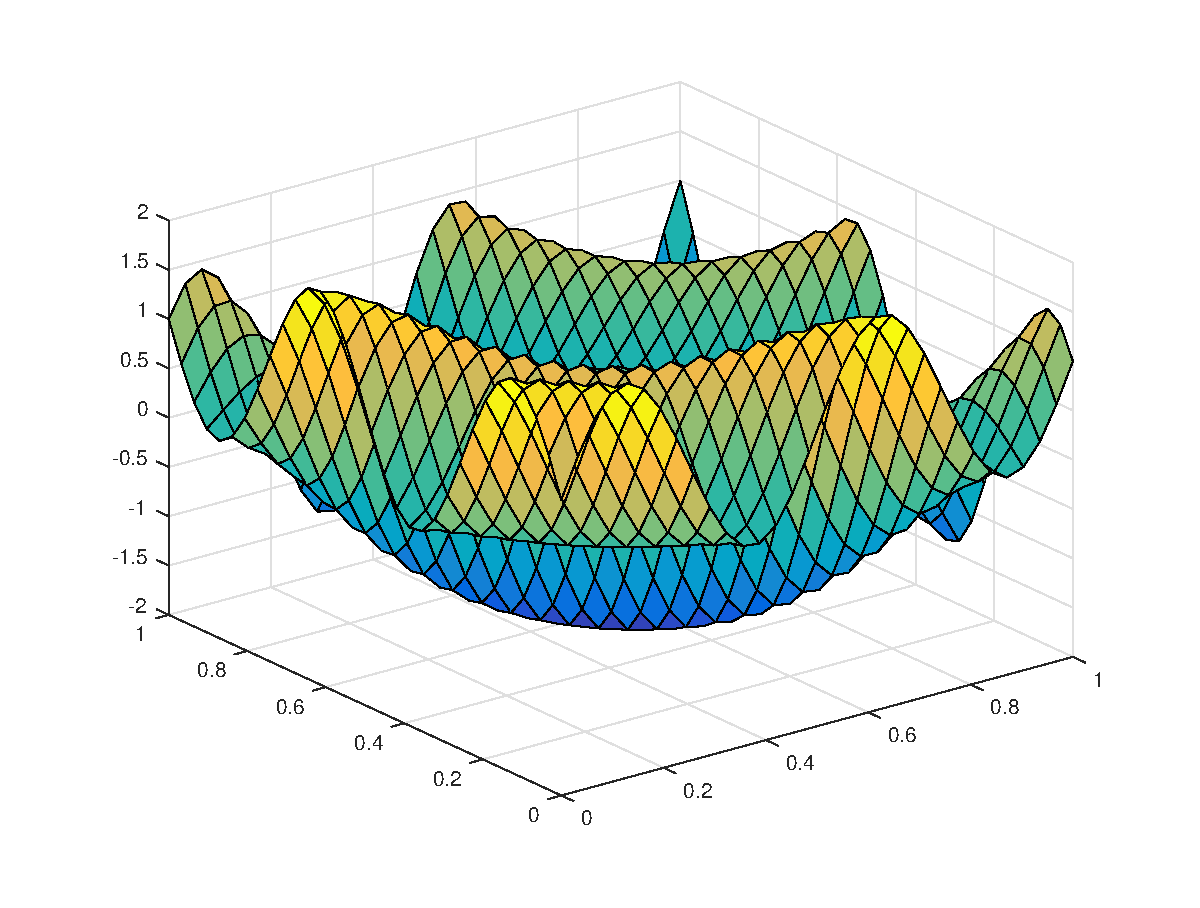
\includegraphics[width=.9\linewidth]{../Figures/ex2u0exact}
  \captionof{figure}{$u_{0,exact}$ on $32 \times 32$ grid}
  \label{fig:ex2:u0exact}
\end{minipage}%
\begin{minipage}{.5\textwidth}
  \centering
  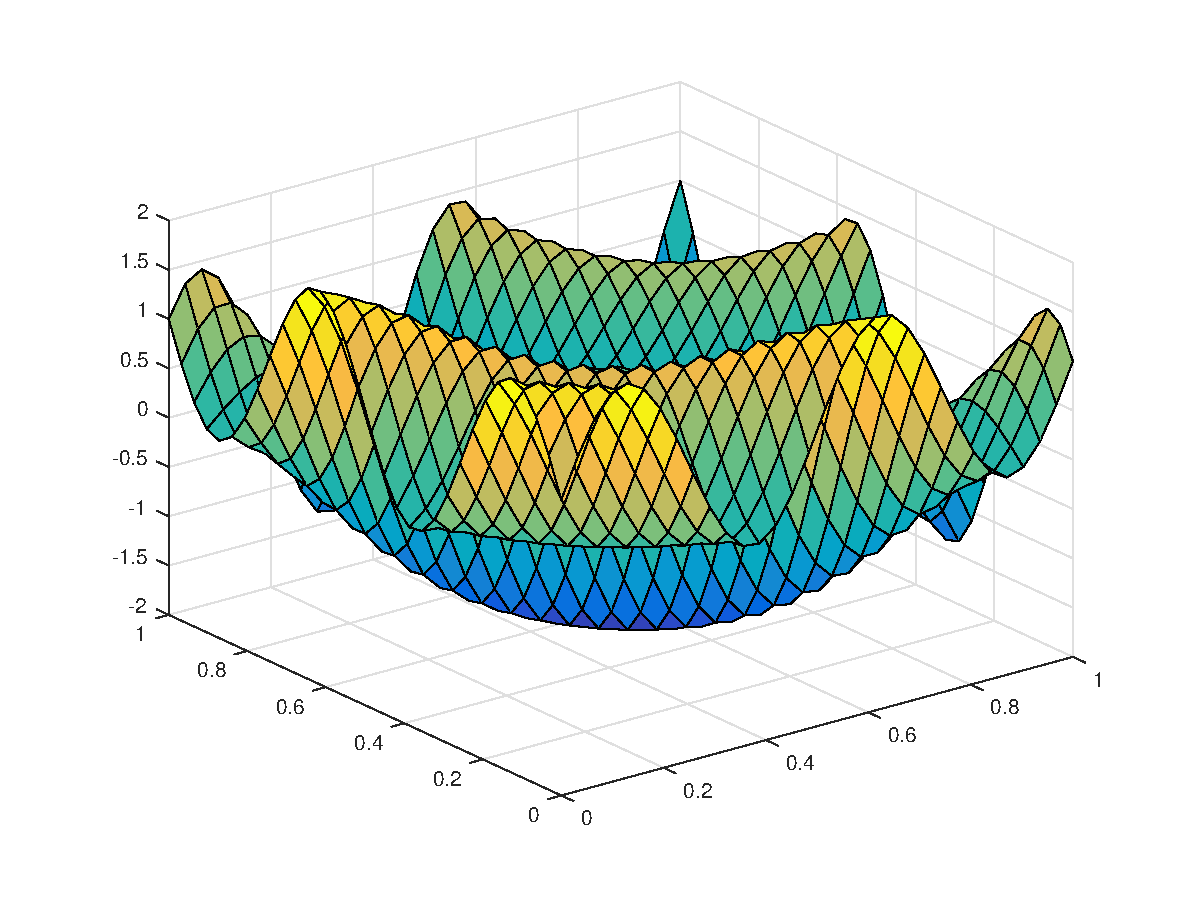
\includegraphics[width=.9\linewidth]{../Figures/ex2u0calc}
  \captionof{figure}{Calculated $u$ using \texttt{poisson9} \textbackslash \texttt{form\_rhs}}
  \label{fig:ex2:u0calc}
\end{minipage}
\end{figure}

% u1
\subsubsection*{Second case}
\begin{align}
    u_{1}(x,y) &= x^2 + y^2 \\
    f_1(x,y) &= 4
\end{align}

\begin{figure}[h]
\centering
\begin{minipage}{.5\textwidth}
  \centering
  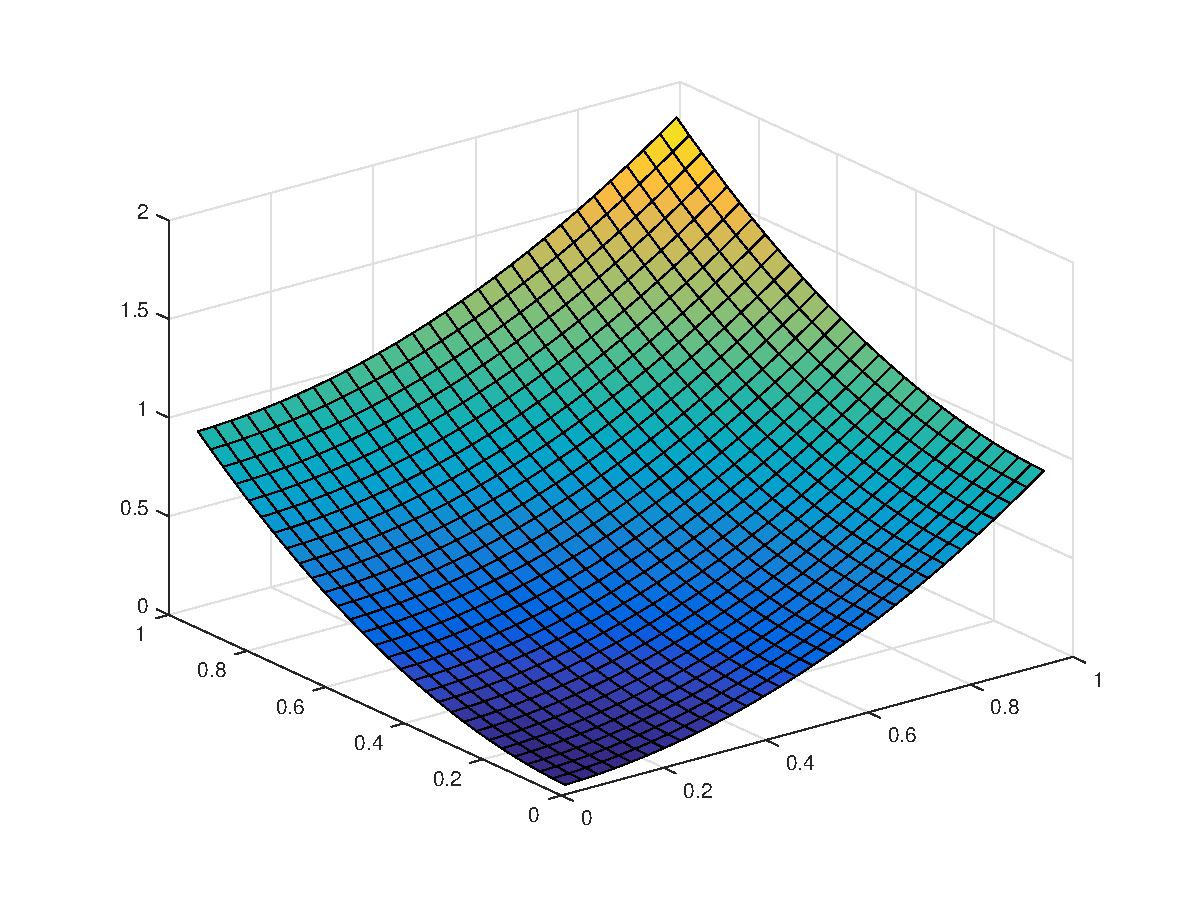
\includegraphics[width=.9\linewidth]{../Figures/ex2u1exact}
  \captionof{figure}{$u_{1,exact}$ on $32 \times 32$ grid}
  \label{fig:ex2:u1exact}
\end{minipage}%
\begin{minipage}{.5\textwidth}
  \centering
  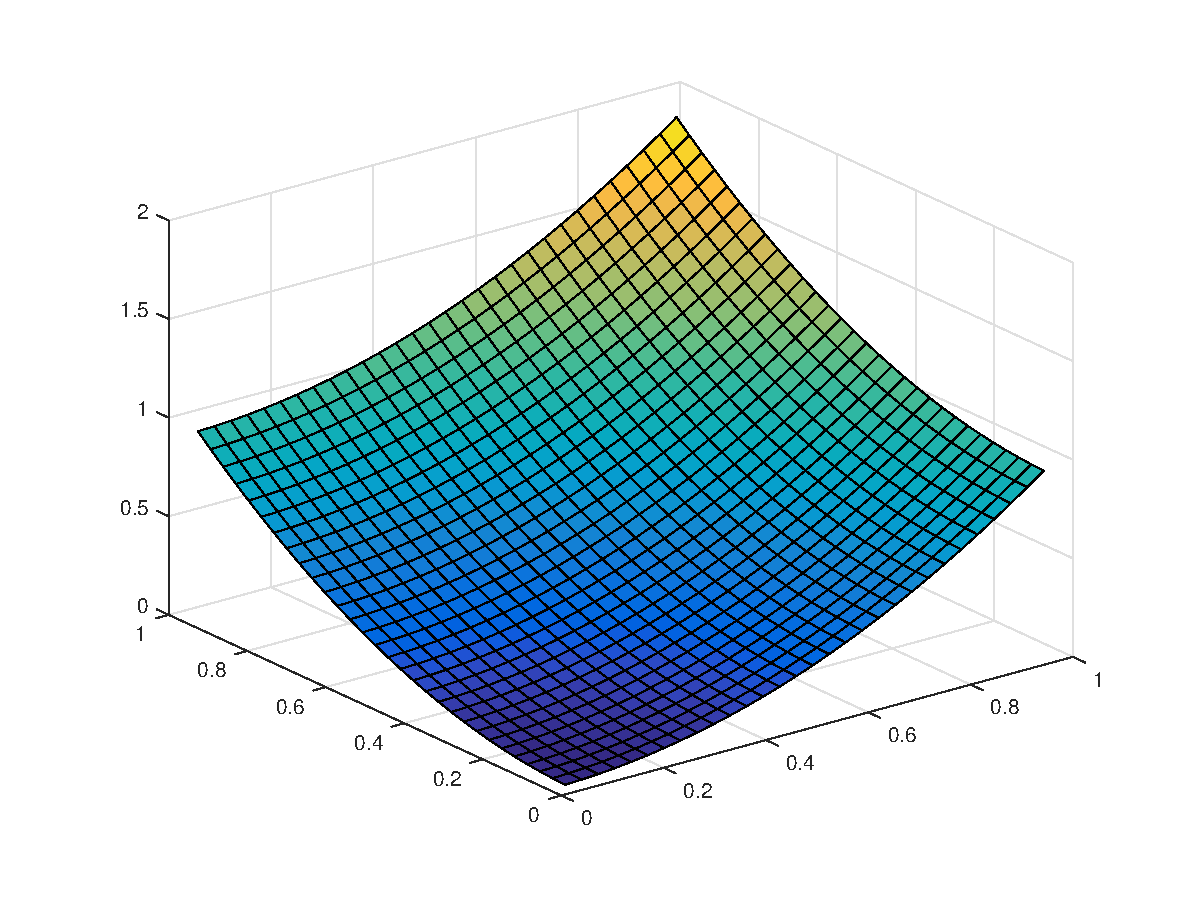
\includegraphics[width=.9\linewidth]{../Figures/ex2u1calc}
  \captionof{figure}{Calculated $u$ using \texttt{poisson9} \textbackslash \texttt{form\_rhs}}
  \label{fig:ex2:u1calc}
\end{minipage}
\end{figure}

% u2
%u2 = @(x,y) sin(2*pi*abs(x - y).^(2.5));
%U2 = u2(X,Y);
%f2 = @(x1,y1) 5*pi*abs(x1 - y1).^(1/2).*sign(x1 - y1).^2.*(...
%    3*cos(2*pi*abs(x1 - y1).^(5/2))...
%    - 10*pi*abs(x1 - y1).^(5/2).*sin(2*pi*abs(x1 - y1).^(5/2))...
%);
\subsubsection*{Third case}
\begin{align}
    u_{2}(x,y) &= \sin(2 \pi |x-y|^{2.5}) \\
    f_2(x,y) &= 5 \pi \sqrt{|x-y|} \sgn(x-y)^2 \left(3 \cos(2 \pi |x-y|^{\frac{5}{2}}) - 10 \pi |x-y|^{\frac{5}{2}} \sin(2 \pi |x-y|^{\frac{5}{2}}) \right)
\end{align}

\begin{figure}[h]
\centering
\begin{minipage}{.5\textwidth}
  \centering
  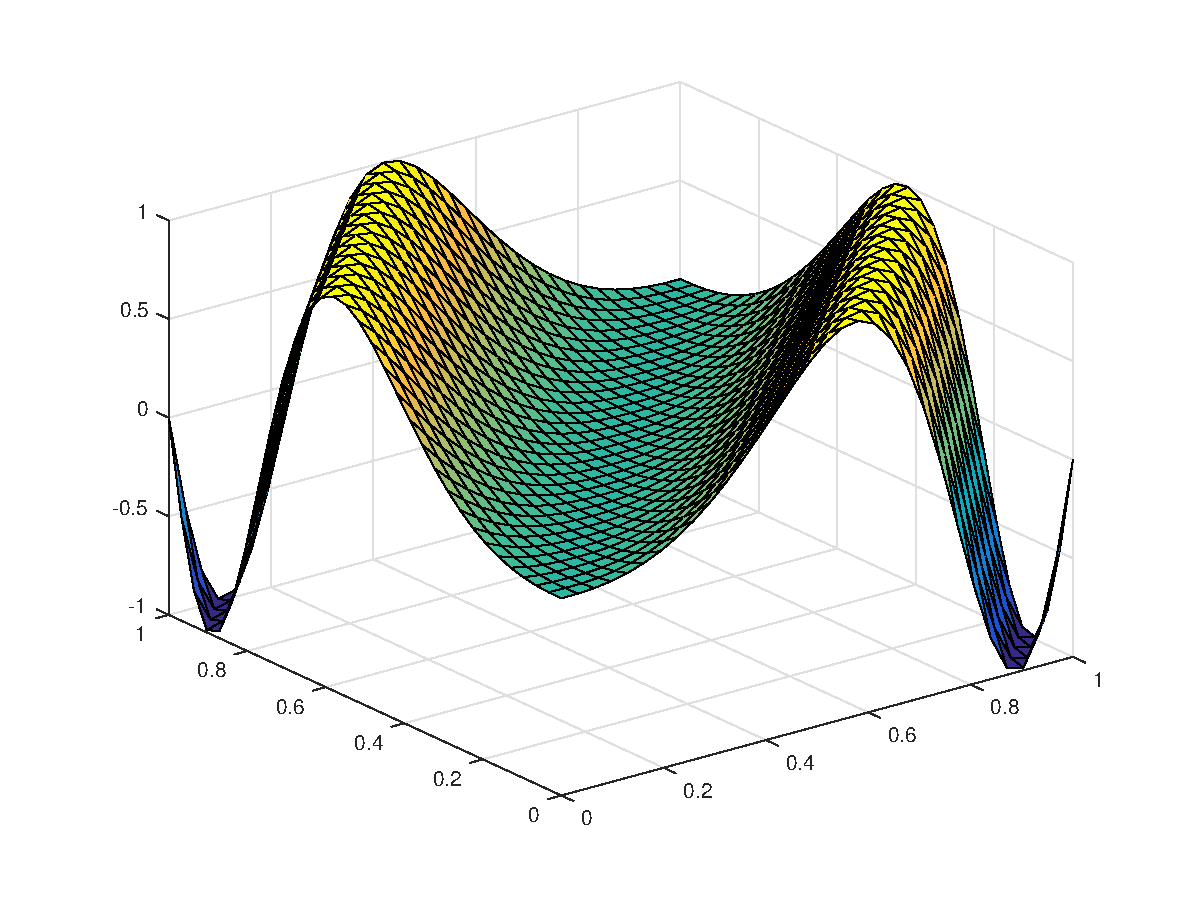
\includegraphics[width=.9\linewidth]{../Figures/ex2u2exact}
  \captionof{figure}{$u_{2,exact}$ on $32 \times 32$ grid}
  \label{fig:ex2:u2exact}
\end{minipage}%
\begin{minipage}{.5\textwidth}
  \centering
  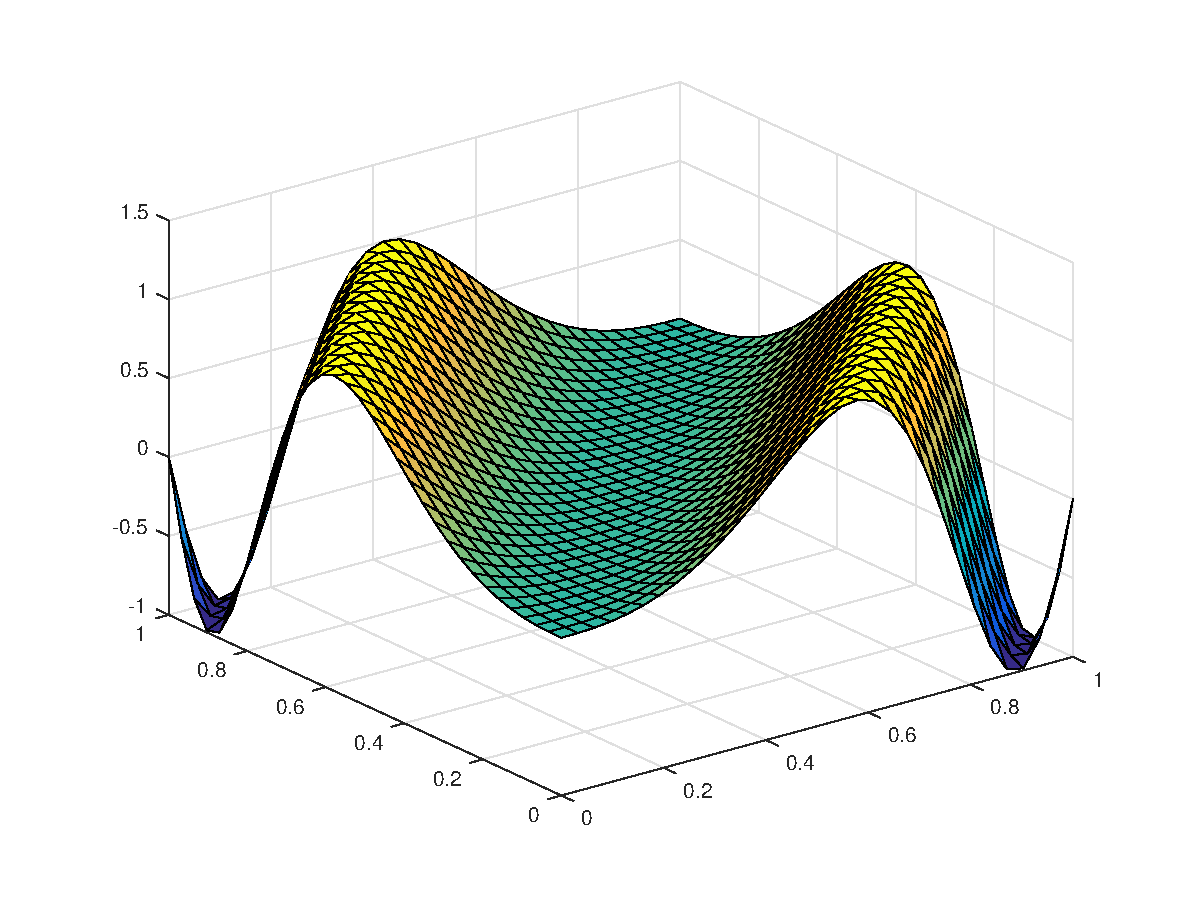
\includegraphics[width=.9\linewidth]{../Figures/ex2u2calc}
  \captionof{figure}{Calculated $u$ using \texttt{poisson9 \textbackslash form\_rhs}}
  \label{fig:ex2:u2calc}
\end{minipage}
\end{figure}


















\end{document}